\documentclass[tikz,border=10pt]{standalone}
\usepackage{tikz}
\usetikzlibrary{positioning,shapes.geometric,arrows.meta,calc}
\usepackage{amsmath}

\begin{document}
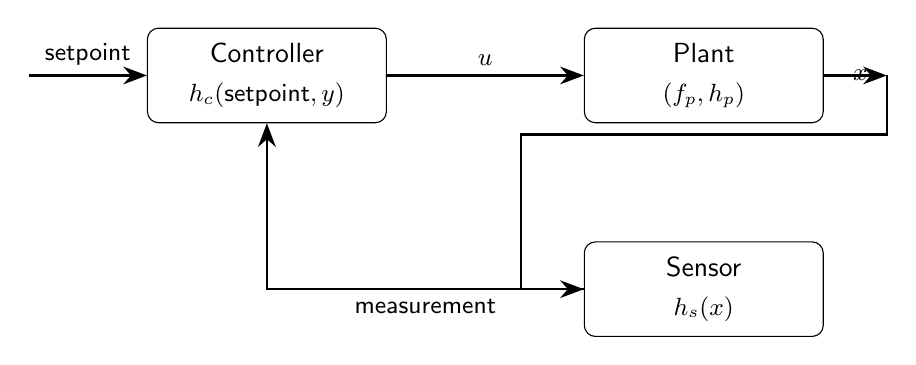
\begin{tikzpicture}[
    node distance=2.5cm,
    block/.style={rectangle, draw, fill=white, text width=2.8cm, text centered, rounded corners, minimum height=1.2cm, font=\sffamily},
    sum/.style={circle, draw, fill=white, minimum size=0.8cm, font=\sffamily},
    arrow/.style={-{Stealth[length=3mm]}, thick},
    signal/.style={font=\small\sffamily}
]

% Blocks
\node[block] (controller) {Controller\\[2pt]{\small $h_c(\text{setpoint}, y)$}};
\node[block, right=of controller] (plant) {Plant\\[2pt]{\small $(f_p, h_p)$}};
\node[block, below=1.5cm of plant] (sensor) {Sensor\\[2pt]{\small $h_s(x)$}};

% Input
\coordinate[left=1.5cm of controller] (input);

% Intermediate coordinates for feedback path
\coordinate[right=0.8cm of plant] (plant_out);
\coordinate[below=0.75cm of plant_out] (feedback_down);
\coordinate[left=0.8cm of sensor] (sensor_in);

% Forward path
\draw[arrow] (input) -- node[above, signal] {setpoint} (controller);
\draw[arrow] (controller) -- node[above, signal] {$u$} (plant);
\draw[arrow] (plant) -- node[right, signal, pos=0.3] {$x$} (plant_out);

% Feedback path
\draw[arrow] (plant_out) |- (feedback_down) -| (sensor_in) -- (sensor);
\draw[arrow] (sensor) -| node[below, signal, pos=0.25] {measurement} ($(controller.south)+(0,-0.5)$) -- (controller.south);

\end{tikzpicture}
\end{document}
